\begin{figure}[ht!]
\centering

\scalebox{0.8}{
\begin{tikzpicture}[auto]

% nodes =============================
\node[box] (ent) {entrada};
\node[box, right=40pt of ent] (NN) {modelo};
\node[box, right=40pt of NN] (saida) {saída};
\node[textonly, right=18pt of saida] (inv1) {};
\node[textonly, below=5pt of inv1] (inv2) {};
\node[box, right=40pt of saida] (saidaesp) {saída \\ esperada};
\node[boxtextonly, below=90pt of inv1] (comp) {Comparação \\ Erro};
\node[boxtextonly, left=70pt of comp] (Uso) {Alteração \\ dos \\ parâmetros};

% edges =============================
\path[tedge, orange!120, line width=1mm] (ent) -- (NN);
\path[tedge, orange!120, line width=1mm] (NN) -- (saida);
\path[tedge, orange!120, line width=0.5mm] (saida) -- (saidaesp);
\path[tedge, orange!120, line width=0.5mm] (saidaesp) -- (saida);
\path[tedge, orange!120, line width=1mm] (inv2) -- (comp);
\path[tedge, orange!120, line width=1mm] (comp) -- (Uso);
\path[tedge, orange!120, line width=1mm] (Uso) -- (NN);


% animation ============================

\visible<2->{\node[textonly, above=5pt of ent] (shirt) {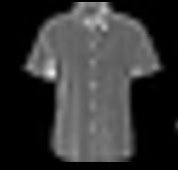
\includegraphics[width=.10\textwidth]{images/shirt.png}};}

\node[textonly, above=8pt of NN] (rede) {Rede Neural};

\visible<3->{\node[textonly, above=8pt of saida] (saida2) {meia};}

\visible<4->{\node[textonly, above=8pt of saidaesp] (saida3) {camiseta};}

\visible<4->{\node[textonly, below=15pt of comp] (mse) {Erro Quadrático Médio};}

%\node[textonly, below=5pt of] () {};

%\node[textonly, below=5pt of] () {};

%\node[textonly, below=5pt of] () {};

%\node[textonly, below=5pt of] () {};

%\node[textonly, below=5pt of] () {};





\end{tikzpicture}
} % scalebox
\end{figure}
